\documentclass[11pt, addpoints, answers]{exam}

\usepackage{amsmath, amssymb}
\usepackage{xcolor}
\usepackage{enumerate}
\usepackage{graphicx}
\usepackage{tabularx}
\usepackage{algorithm}
\usepackage{algpseudocode}
\usepackage{tikz}
\usepackage{tikz-qtree}
\usepackage{subfigure}
\usetikzlibrary{positioning}
\usetikzlibrary{graphs}
\usetikzlibrary{arrows.meta}

\newcommand{\red}[1]{\textcolor{red}{#1}}
\newcommand{\blue}[1]{\textcolor{blue}{#1}}

% For inserting code snippets.
\usepackage{listings}
\lstset{
    columns = fixed,
    numbers=left,
    basewidth = {0.5em},
    breaklines = true,
    backgroundcolor = \color{white},
    keywordstyle = \color[RGB]{40, 40, 255},
    numberstyle = \footnotesize\color{darkgray},
    commentstyle = \ttfamily\color{violet},
    basicstyle = \ttfamily,
    stringstyle = \ttfamily\color[RGB]{128, 0, 0},
    showstringspaces = false,
    language = {[11]C++},
    escapechar = \@
}
\lstnewenvironment{cpp}[1][]{\lstset{language = {[11]C++}, #1}}{}

\renewcommand{\baselinestretch}{1.15}
\setlength{\parskip}{1.25\baselineskip}

\usepackage{tikz}
\usepackage{tikz-qtree}
\tikzset{every tree node/.style={minimum width=2em,draw,circle},
    blank/.style={draw=none},
    edge from parent/.style=
    {draw,edge from parent path={(\tikzparentnode) -- (\tikzchildnode)}},
    level distance=1.2cm}


% headers, footers, titles
\newcommand{\CourseName}{CS101 Algorithms and Data Structures}
\newcommand{\HomeworkNO}{11}
\newcommand{\DueDate}{December 22, 2024}

\pagestyle{headandfoot}
\runningheadrule
\runningheader{CS101 Fall24}{Homework \HomeworkNO}{Due on: \DueDate}
\runningfooter{}{\thepage}{}

\title{
    \vspace{25pt}
    \LARGE ShanghaiTech University \\
    \bigskip
    \textbf{\CourseName} \\
    \textbf{Fall 2024}   \\
    \bigskip
    Homework \HomeworkNO
}
\author{}
\date{Due date: \DueDate, at 23:59}

% formats of questions, choices, points, etc.
\qformat{\bf\thequestion. (\totalpoints\ points) \thequestiontitle\hfill}
\pointname{'}
\bonuspointname{' (bonus)}
% \CorrectChoiceEmphasis{\bf\color{blue}}
% \SolutionEmphasis{\color{blue}}

% We frequently use this font.
\newcommand{\ttt}{\texttt}
\newcommand{\bluett}[1]{\textcolor{blue}{\ttt{#1}}}

\newcommand*{\TrueFalse}[1]{%
\ifprintanswers
    \ifthenelse{\equal{#1}{T}}{
        \hfill \parbox[t]{1.50in}{\begin{oneparcheckboxes} \CorrectChoice True \choice False \end{oneparcheckboxes}}
    }{
        \hfill \parbox[t]{1.50in}{\begin{oneparcheckboxes} \choice True \CorrectChoice False \end{oneparcheckboxes}}
    }
\else
    \hfill \parbox[t]{1.50in}{\begin{oneparcheckboxes} \choice True  \choice False \end{oneparcheckboxes}}
\fi
} 


\begin{document}

\maketitle

\vspace{50pt}

\begin{enumerate}
    \item Please write your solutions in English.
    \item Submit your solutions to Gradescope.
    \item Set your FULL name to your Chinese name and your STUDENT ID correctly in Gradescope account settings.
    \item If you want to submit a handwritten version, scan it clearly. \ttt{CamScanner} is recommended.
    \item We recommend you to write in \LaTeX.
    \item When submitting, match your solutions to the problems correctly.
    \item No late submission will be accepted.
    \item Violations to any of the above may result in zero points.
\end{enumerate}
\newpage

{\large\textbf{Demand of the Algorithm Design:}} \textcolor{red}{(MUST READ! )}

All of your algorithms should need the three-part solution, this will help us to score your algorithm. You should include {\large\textbf{main idea,  proof of correctness and run-time analysis.}} The detail is as below:
\begin{enumerate}
\item The {\textbf{main idea}} of your algorithm. You should correctly convey the idea of the algorithm in this part. It does not need to give all the details of your solutions or explain why they are correct. When grading these problems, we will emphasize how you define your sub-problems, whether your Bellman equation is correct, and the correctness of your complexity analysis:
    \begin{enumerate}
        \item \textbf{Define your subproblems clearly.} Your definition should include the variables you choose for each subproblem and a brief description of your subproblem in terms of the chosen variables. 
        \item Your \textbf{Bellman equation} should be a recurrence relation whose \textbf{base case} is well-defined.
        \item You can \textbf{briefly explain each term in the equation} if necessary, which might improve the readability of your solution and help us grade it.
    \end{enumerate}
\item A {\textbf{proof of correctness}}.  You must prove that your algorithm work correctly, no matter what input is chosen. For iterative or recursive algorithms, often a useful approach is to find an invariant. A loop invariant needs to satisfy three properties: (1) it must be true before the first iteration of the loop; (2) if it is true before the $i$th iteration of the loop, it must be true before the $i$ + 1st iteration of the loop; (3) if it is true after the last iteration of the loop, it must follow that the output of your algorithm is correct. You need to prove each of these three properties holds. Most importantly, you must specify your invariant precisely and clearly. \textbf{However, sometimes the problem does not require you to prove the correctness of your algorithm. But remember to give your bellman Equation clearly.}
If you invoke an algorithm that was proven correct in class, you don’t need to re-prove its correctness.
\item The asymptotic \textbf{running time} of your algorithm, stated using $\Theta$(·) notation. And you should have your \textbf{running time analysis}, i.e., the justification for why your algorithm’s running time is as you claimed. Often this can be stated in a few sentences (e.g.: “the loop performs $|E|$ iterations; in each iteration, we do $\Theta(1)$ Find and Union operations; each Find and Union operation takes $\Theta(\log|V|)$ time; so the total running time is $\Theta(|E|\log|V|)$”). Alternatively, this might involve showing a recurrence that characterizes the algorithm’s running time and then solving the recurrence.

\item You only need to calculate the optimal value in each problem of this homework and you don’t have to back-track to find the optimal solution.
\end{enumerate}

\begin{questions}

% \titledquestion{Multiple Choices}

Each question has \textbf{one or more} correct answer(s). Select all the correct answer(s). For each question, you will get 0 points if you select one or more wrong answers, but you will get 1 point if you select a non-empty subset of the correct answers.

Write your answers in the following table.

%%%%%%%%%%%%%%%%%%%%%%%%%%%%%%%%%%%%%%%%%%%%%%%%%%%%%%%%%%%%%%%%%%%%%%%%%%%
% Note: The `LaTeX' way to answer a multiple-choice question is to replace `\choice'
% with `\choice', as what you did in the first question. However, there are still
% many students who would like to handwrite their homework. To make TA's work easier,
% you have to fill in your selected choices in the table below, no matter whether you use 
% LaTeX or not.
%%%%%%%%%%%%%%%%%%%%%%%%%%%%%%%%%%%%%%%%%%%%%%%%%%%%%%%%%%%%%%%%%%%%%%%%%%%

\begin{table}[htbp]
	\centering
	\begin{tabular}{|p{2cm}|p{2cm}|p{2cm}|p{2cm}|p{2cm}|}
		\hline 
		(a) & (b) & (c) & (d) & (e) \\
		\hline
  		%%%%%%%%%%%%%%%%%%%%%%%%%%%%%%%%%%%%%%%%%%%%%%%%%%%%%%%%%%
		% YOUR ANSWER HERE.
		   &  &  &  &  \\
            %%%%%%%%%%%%%%%%%%%%%%%%%%%%%%%%%%%%%%%%%%%%%%%%%%%%%%%%%%
		\hline
	\end{tabular} 
\end{table}

\begin{parts}


\part[2] Which of the following statement(s) is/are true for an AVL tree?
\begin{choices}
    \choice Inserting an item can unbalance non-consecutive (not directly connected) nodes on the path from the root to the inserted item before the restructuring.
    \choice Inserting an item can cause at most one node imbalanced before the restructuring.
    \choice Only at most one node-restructuring has to be performed after inserting an item.
    \choice Removing an item in leaf nodes can cause at most one node imbalanced before the restructuring. 
    
\end{choices}

\part[2] Consider an AVL tree whose height is h, which of the following is/are true? 

\begin{choices}

\choice This tree contains $\Omega(\alpha^h)$ nodes, where $\alpha = \dfrac{\sqrt{5}-1}{2}$.

\choice This tree contains $\Theta(2^h)$ nodes.

\choice This tree contains $O(h)$ nodes in the worst case.

\choice None of them above.

\end{choices}

\part[2]  Which of the following about the comparison between AVL-tree and BST is/are true? Suppose $n$ is the number of nodes in the tree.

\begin{choices}
    
    \choice The cost of searching an AVL tree is $O(\log n)$ but that of a complete binary search tree is $O(n \log n)$.

    \choice The cost of searching an AVL tree is $\Theta(\log n)$ but that of a binary search tree is $O(n)$.
    
    \choice The cost of searching a binary search tree with height h is $O(h)$ but that of an AVL tree is $O(\log n)$.
    
    \choice The corrections of both Insertion and Erasion cost $\Theta(\log n)$ time in worst cases in an AVL tree.

\end{choices}

\part[2] Which of the following statements is/are true for an AVL tree? Here one balance correction means a single rotation (in left-left or right-right cases) or a double rotation (in left-right or right-left cases). 

\begin{choices}
    \choice In an AVL tree, during the insert operation there are at most two rotations needed.
    \choice Inserting an item causes at most one node imbalance before checking if any balance correction is needed.
    \choice At most one balance correction has to be performed after inserting an item.
    \choice At most one balance correction has to be performed after removing an item.
\end{choices}

\part[2] You are given an AVL tree as a blow. Suppose we promote the minimum element in the right sub-tree when erasing a node with 2 children. Which of the following operation sequences will cause 2 imbalances that must be corrected in total in order to rebalance the tree?

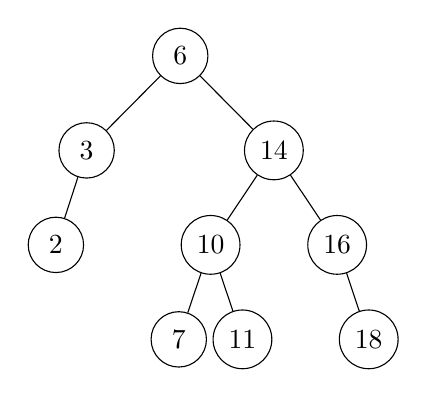
\begin{tikzpicture}
\Tree
[.6
    [.3
        \edge[];[.2
        ]
        \edge[blank]; \node[blank]{};
    ]
    [.14
        \edge[];[.10
            \edge[];[.7
            ]
            \edge[];[.11
            ]
        ]
        \edge[];[.16
            \edge[blank]; \node[blank]{};
            \edge[];[.18
            ]
        ]
    ]
]
\end{tikzpicture}

\begin{choices}
    \choice Erase $2$, $6$.
    \choice Insert $4$, $5$, $12$. Erase $2$.
    \choice Erase $6$, $2$, $3$. Insert $20$.
    \choice Insert $1$, $0$, $4$, $13$, $19$.
\end{choices}

\end{parts} 

\newpage


\titledquestion{(DP Example) Maximum Subarray Problem}

\vspace{0.1in}

Given an array $A=\langle A_1, \dots, A_n\rangle$ of $n$ elements, please design a dynamic programming algorithm to find a contiguous subarray whose sum is maximum.

% utilities you might need for wrting Bellman equations
\newcommand{\maxi}[2]{\max\left\{\substack{#1\\#2}\right\}}	% usage: \maxi{a}{b}
\newcommand{\mini}[2]{\min\left\{\substack{#1\\#2}\right\}}	% usage: \mini{a}{b}
\newcommand{\case}[1]{\text{if}\ #1}	% usage: \case{$i > 1$}
\newcommand{\otherwise}{\text{otherwise}}	% usage: \otherwise


\begin{solution}

    \textbf{Main Idea}
    
    Let $OPT(I)$ be the maximum sum of subarrays of $A$ ending with $A_i$. 
    Then we have the following equation:
    \[
    OPT(i)=
    \begin{cases}
        A_1                       & \case{i=1} \\
        \max \{A_i,A_i+OPT(i-1)\} & \otherwise
    \end{cases}
    \]

    The final answer is 
    \[ \max_{i\in\{1, 2, \dots, n\}} OPT(i) \]

    \textbf{Proof of Correctness}: 

    \begin{itemize}
        \item The $1$st term in $\max$: only take $A_i$
        \item The $2$nd term in $\max$: take $A_i$ together with the best subarray ending with $A_{i-1}$
    \end{itemize}

    \textbf{Runtime Analysis}: 

    The running time is $\Theta(n)$ since we have a single loop with range $n$ to reduce subproblems.
\end{solution}

\titledquestion{Odd number of coins changing}[8]

Given n coin denominations $\{c_1,c_2,\cdots,c_n\}$ and a target value $V$, you are going to make change for $V$. However, only odd number of coins is allowed.

Please design a \textbf{dynamic programming} algorithm that find the fewest odd number of coins needed to make change for $V$ (or report impossible).

\textbf{Hints:} \textit{For this problem, you can formulate your subproblems as:}
\begin{center}
    $F(v)=$ fewest odd number of coins to make change for $v$.
    
    $G(v)=$ fewest even number of coins to make change for $v$.
\end{center}

\begin{solution}
    \vspace{6in}
    
\end{solution}


\titledquestion{Happiness Planning}[10]

In the magical world of Hogwarts, Professor Slughorn likes to plan his potions classes with precision and flair.

For the next \( m \) months, starting with no Galleons, Slughorn will brew potions and earn \( x \) Galleons per month. During the \( i \)-th month (\( 1 \leq i \leq m \)), there will be a singular chance to spend \( c_i \) Galleons to acquire happiness worth \( h_i \). However, it's a fair bargain for Slughorn to buy happiness, that is, the amount of $c_i$ will not be too big.

Borrowing is not permitted. Galleons earned in the \( i \)-th month can only be used in a subsequent \( j \)-th month (\( j > i \)).

Since potion masters don't dabble with Muggle technology, please help him design a dynamic programming algorithm to assist Slughorn in discovering the maximum achievable sum of happiness.

\textbf{Hints: } \textit{Still consider the backpack problem! What should you design the Bellman equation with limitation?}

\begin{solution}
    \vspace{5in}
    
\end{solution}
\titledquestion{Greedy doesn't work}
Tom and Jerry are playing an interesting game, where there are $n$ cards in a line. All cards are faced-up and the number on every card is between 2-9. Tom and Jerry take turns. In anyone's turn, they can take one card from either the right end or the left end of the line. The goal for each player is to maximize the sum of the cards they have collected.


\begin{parts}
\part[3] Tom decides to use a greedy strategy: ``On my turn, I will take the larger of the two cards available to me." Show a small counterexample ($n\leq 5$) that Tom will lose if he plays this greedy strategy. Assuming Tom goes first and Jerry plays optimally. Tom could have won if he also played optimally.

\begin{solution}
    \vspace{1in}
    
\end{solution}

\part[7] Jerry decides to use dynamic programming to find an algorithm to maximize his score, assuming he is playing against Tom and Tom is using the greedy strategy from part (a). Help Jerry to develop the dynamic programming solution. The solution you proposed should not worse than $O(n^2)$ in time complexity.

\begin{solution}
    \vspace{3.5in}
    
\end{solution}
\end{parts}

\titledquestion{Pairwise DNA Sequence Alignment}

\newcommand{\maxt}[3]{\max\begin{cases}#1\\#2\\#3\end{cases}}

Given two DNA sequences: a query sequence $Q=\langle Q_1, \dots, Q_m\rangle$ of $m$ nucleotides and a subject sequence $S=\langle S_1, \dots, S_n\rangle$ of $n$ nucleotides. There are $4$ types of nucleotides, namely Adenine (A), Cytosine (C), Guanine (G) and Thymine (T). We provide a scoring matrix for nucleotides at the same index of these two sequences:


\begin{table}[!htbp]
	\centering
	\begin{tabular}{|c|c|c|c|c|} \hline
		  & A  & C  & G  & T  \\ \hline
		A & 1  & -5 & -1 & -5 \\ \hline
		C & -5 & 1  & -5 & -1 \\ \hline
		G & -1 & -5 & 1  & -5 \\ \hline
		T & -5 & -1 & -5 & 1  \\ \hline
	\end{tabular}
\end{table}


where $\text{Score}(X, X)$ on the diagonal represents the score of a successful match for nucleotide $X$ at the same index of both sequences, and  $\text{Score}(X, Y)$ indicates the penalty for mismatching nucleotide $X$ by nucleotide $Y$.


For example, assume we have $m=n$ here and there are two sequences $Q=\langle TGGTG\rangle$ and $S=\langle ATCGT\rangle$. Then the alignment score for these two sequences is
\[
	\begin{aligned}
		\text{Score}(Q, S) & = \sum_{i}^{n} \text{Score}(Q_i, S_i) \\
		                   & = \text{Score}(T, A)+\text{Score}(G, T)+\text{Score}(G, C)+\text{Score}(T, G)+\text{Score}(G, T) \\
		                   & = (-5)+(-5)+(-5)+(-5)+(-5) \\
		                   & = -25
	\end{aligned}
\]


However, if $m \neq n$, we must insert several gaps `$-$' to make two sequences the same length. In order to align two sequences for higher scores, we can also insert an arbitrary number of gaps `$-$' to each sequence at an arbitrary index. However, adding one gap will result in a gap penalty $\text{Penalty}(X, -)=\text{Penalty}(-, Y)=-2$.


Assume after inserting $4$ gaps, we obtain $Q^\prime=\langle -T-GGTG\rangle$ and $S^\prime=\langle ATCG-T-\rangle$. Then the recomputed alignment score is:
\[
	\begin{aligned}
		\text{Score}(Q^\prime, S^\prime) & = \text{Penalty}(-, A) +\text{Score}(T, T)+\text{Penalty}(-, C) + \text{Score}(G, G) \\
		                                 & \ \ \  +\text{Penalty}(G, -)+\text{Score}(T, T)+ \text{Penalty}(G, -)               \\
		                                 & = (-2)+1+(-2)+1+(-2)+1+(-2)                                                          \\
		                                 & = -5
	\end{aligned}
\]
Notice that $Q^\prime$ and $S^\prime$ should share the same length after inserting gaps.


Given the scoring matrix and gap penalty, please come up with a dynamic programming algorithm to \textbf{maximize the pairwise alignment score} of a pair of DNA sequences by inserting gaps into these two sequences.


\newpage
\begin{parts}
	\part[2] Define your subproblem for this question.
	\begin{solution}
            \vspace{1in}
        \end{solution}


	\part[6] Give your Bellman equation to solve the subproblems. (Proof of correctness is not required)
	\begin{solution}
            \vspace{3in}
        \end{solution}


	\part[1] What is the answer to this question in terms of the subproblems?
	\begin{solution}
            \vspace{0.7in}
        \end{solution}


	\part[1] What is the runtime complexity of your algorithm?
	\begin{solution}
            \vspace{0.7in}
        \end{solution}
\end{parts}

\titledquestion{Pizza Partitioning}

Logan and his good friend Joel want to share a round pizza pie that has been cut into $2n$ equal sector slices along rays from the center at angles $\alpha_i = \frac{i\pi}{n}$ for $i \in \{0,1,...., 2n\}$, where $\alpha_0 = \alpha_{2n}$. Each slice $i$ between angles $\alpha_i$ and $\alpha_{i+1}$ has a known integer tastiness $t_i$ (which might be negative). To be “fair” to her friend, Logan decides to eat slices in the following way:
\begin{itemize}
    \item They will each take turns choosing slices of pizza to eat: Logan starts as the chooser.
    \item If there is only one slice remaining, the chooser eats that slice, and eating stops.
    \item Otherwise the chooser does the following:
    \begin{itemize}
        \item Angle $\alpha_i$ is proper if there is at least one uneaten slice on either side of the line passing
through the center of the pizza at angle $\alpha_i$.
        \item The chooser picks any number $i \in \{1,...,2n\}$ where $\alpha_i$ is proper, and eats all uneaten slices counter-clockwise around the pizza from angle $\alpha_i$ to angle $\alpha_i + \pi$.
    \end{itemize}
\end{itemize}

Logan wants to maximize the total tastiness of the slices she will eat. Describe an $O(n^3)$-time dynamic programming algorithm
to find the maximum total tastiness Logan can guarantee herself via this selection process. 

\textbf{Hints}: \textit{As they eat pizza, the uneaten slices are always cyclically consecutive. That is, each time the chooser eats all uneaten slices within half side, There is no chance that two consecutively parts of pizza are left uneaten. You can choose consecutive cyclic subarrays as the subproblems.}

\begin{figure}[htbp]
    \centering
    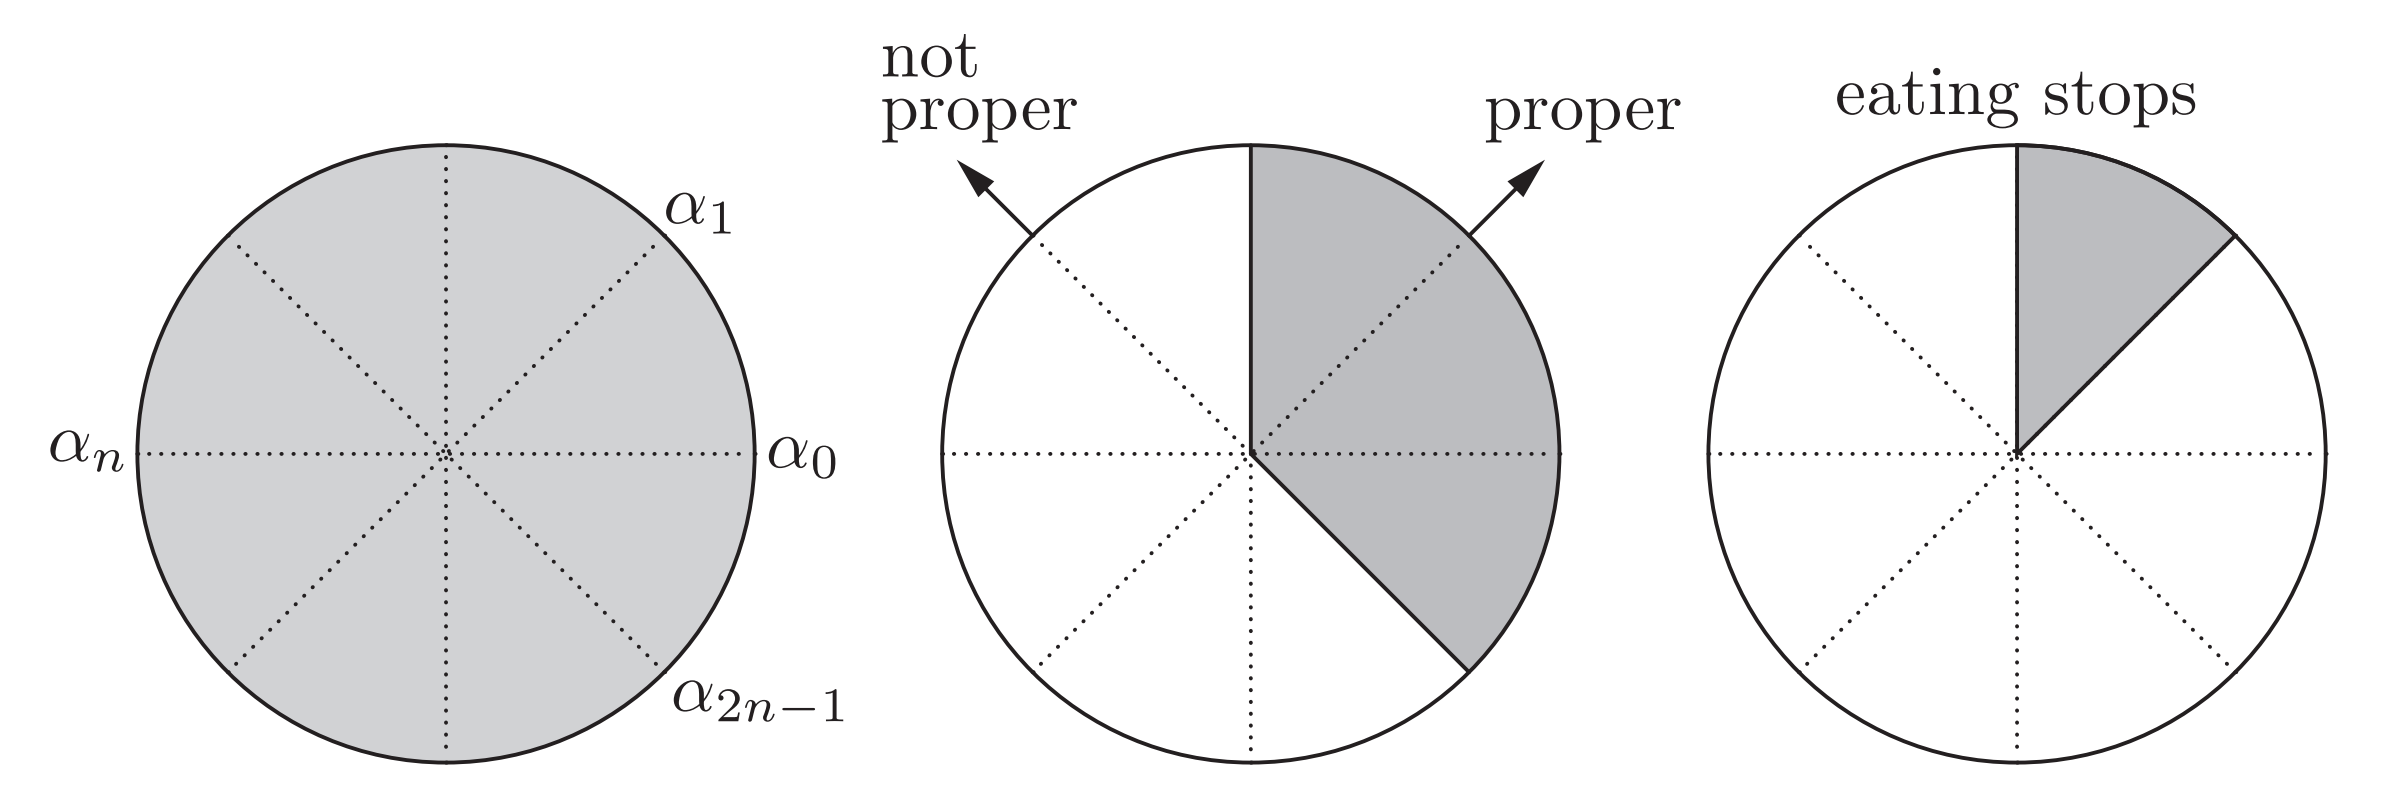
\includegraphics[width=1\linewidth]{p6.png}
\end{figure}

\begin{parts}
    \part[2] As a kickoff, let $v(i, j)$ be the tastiness of the $j$ slices counter-clockwise from angle $\alpha_i$. Write the formula over $v(i, j)$. 

    \begin{solution}
        \vspace{1in}
    \end{solution}

    \part[2] Define your subproblem for this question.

    \begin{solution}
        \vspace{1in}
    \end{solution}

    \bonuspart[4] Give your Bellman equation to solve the subproblems. (Proof of correctness is not required) 

    \begin{solution}
        \vspace{4in}
    \end{solution}

    \bonuspart[2] What is the answer to this question in terms of the subproblems?

    \begin{solution}
        \vspace{1in}
    \end{solution}

    \newpage

    \bonuspart[2] Give an explanation and time complexity analysis of this algorithm.
    \begin{solution}
        \vspace{8in}
    \end{solution}

    
\end{parts}

\end{questions}

\end{document}